
Abychom mohli hovořit o konkrétních technologiích, musíme nejdříve definovat základní technologické stavební kameny, o které se BigData opírají. Jedná se o technologie a paradigmata vyvinutá technologickými giganty, kteří jako první naráželi na technologické hranice a posouvali je dál. Pořadí těchto technologií a paradigmat se odvíjí od logické posloupnosti tak, jak spolu souvisí a navazují na sebe.    

\section{Distribuované systémy}
Distribuované systémy jsou tématem, které zasahuje samozřejmě mnohem dále než jen do oblasti BigData. Pro zjednodušení následujících řádků zavedeme následující rozdělení: Distribuované systémy rozdělíme na systémy s distribuovaným výpočetním výkonem, systémy s distribuovaným úložištěm anebo kombinaci obojího. 

Distribuovaný výpočetní výkon je takový systém, kde se výpočet jedné úlohy rozloží na více počítačů. Paralelní výpočty jsou známé z oblasti informačních technologií již mnoho let a používají se nejčastěji k vědeckým výpočtům, paralelní kompilaci zdrojových kódů anebo k jiným operacím, které by na jednom počítači trvaly příliš dlouho. 

Distribuované úložistě je jednoduše představitelné a důvodů mít data na více místech je hned několik.
\begin{itemize}
\item Záloha - i ze sféry osobních počítačů známe trend, kdy máme data zálohovaná na více fyzických zařízeních, abychom předešli jejich ztrátě v případě technické poruchy na daném zařízení. 

\item Nedostatek kapacity - Ze sféry osobních počítačů známe, že uživatelé méně potřebné soubory ukládají na externí periferie, protože kapacita disků v osobních počítačích je zpravidla v řádu stovek GB.

\item Dostupnost - Pokud chce uživatel mít přístup k jednomu souboru z domácího i pracovního počítače, musí se tento soubor fyzicky nacházet na obou počítačích nebo musí využít nějaký software na sdílení souborů. 

\end{itemize}

Kombinovaný přístup je zřejmý. Používá se jak výpočetní výkon jednotlivých počítačů v systému, tak jejich úložný prostor. 

BigData využívá všechny tyto přístupy. Je zřejmé, že obrovské množství dat, o kterém jsme mluvili v úvodu, se lépe zpracovává na více počítačích. Stejně tak je logické, že velké množství dat uložíme na více počítačů a to platí i v případě, že chceme data zálohovat. 

Ne vždy však využíváme kombinovaný přístup. Je totiž velmi časté, že si firmy staví obrovské počítačové farmy, které slouží pouze jako datové sklady a datová centra. Vždy záleží na konkrétní situaci a způsobu využití. 


\section{CAP Theorem}
 Při nástupu distribuovaných systémů v roce 2000 vydal vědec Eric Brewer článek popisující tzv. CAP Theorem \cite{cap}, který se distribuovaných systémů přímo týká. Tento teorém říká, že distribuované systémy mají tyto 3 hlavní vlastnosti: 

\begin{itemize}
\item Konzistence (Consistency) - Vlastnost, která určuje, zda pro každý požadavek vrátí server správný výsledek. To znamená, že odpověď je adekvátní vůči specifikaci požadované služby. Přesný význam konzistence se odvíjí od typu služby. V případě dat ji definujeme tak, že každý server má aktuální a stejná data.

\item Dostupnost (Availability) - Vlastnost, která říká, že na každý požadavek dostaneme odpověď. Rychlejší odpověď je preferovanější oproti pomalejší, ale v kontextu teorému je důležité, že odpověď vůbec dorazí. Z praxe však víme, že velice opožděná odpověď je stejně špatná jako žádná odpověď. Můžeme tedy tuto vlastnost zjednodušit a říci, že systém musí být vždy dostupný.

\item Tolerance výpadku (Partiotion tolerance) - Tato vlastnost (jako jediná) určuje chování podpůrného systému, na kterém služba běží, namísto popisu chování služby samotné. Tato vlastnost říká, jestli během výpadku nějaké části systému je tento systém schopný pokračovat a dále fungovat.

\end{itemize}


Brewer popisuje, že každý distribuovaný systém může splňovat nejvýše 2 z těchto 3 vlastností.

\subsection{CAP Theorem v roce 2012}
V roce 2012 napsal Brewer další článek \cite{cap2}, ve kterém popisuje stav jeho teorému po 12 letech. Vysvětluje, že již od začátku bylo označení \uv{pouze 2 ze 3} zavádějící a vágní, protože spoustu věcí příliš zjednodušovalo. Například u systému s velkou granularitou se mezi volbou C a A rozhoduje na několika úrovních a všechny vlastnosti mají spíše hodnoty v čase a ne hodnoty binární a dále také, že záleží na stavbě systému a jeho drobných nuancích. Zároveň však píše, že ve svém důsledku teorém splnil svůj účel a otevřel systémovým návrhářům oči při navrhování distribuovaných systémů a donutil je se zamyslet nad výhodami a nevýhodami jednotlivých vlastností systému. 

V témže roce vyšel další zajímavý článek popisující aktuální stav CAP teorému \cite{cap3}. Popisuje převážně vztah
systémů k volbám CAP vlastností. 

\subsubsection{Nejlepší možná dostupnost}
Nejčastějším výběrem je garantovaná konzistence s maximální možnou dostupností. Pro většinu systémů je to přirozená volba. Server tedy  za každou cenu vrací správnou odpověď a snaží se poté optimalizovat co nejvyšší dostupnost a nejkratší možnou dobu odpovědi vzhledem k síťovým podmínkám. Tento přístup dává největší smysl, pokud jsou počítače ve stejném datacentru a běží na nich stejná služba. Typickým zástupcem je \uv{lock service} a služba spravující metadata pro nějaký distribuovaný systém s nízkou granularitou.

\subsubsection{Nejlepší možná konzistence} 
Druhou nejčastější skupinou jsou systémy, pro které je ztráta dostupnosti nemyslitelná a tudíž ji garantují a snaží se o co nejvyšší úroveň konzistence. Tento postup nejlépe vyhovuje v situacích, kdy máme počítače distribuované napříč několika datacentry. V tomto případě může totiž dostupnost rapidně klesat s jakoukoliv chybou, a proto je potřeba ji garantovat. V těchto případech tedy designéři obětují konzistenci, aby mohli garantovat dostatečně rychlou odpověď, přestože ta nemusí být vždy zcela správná. Ideálním příkladem jsou webové cache a obrázkové servery.

\subsubsection{Segmentovaná konzistence a dostupnost}
Toto je nejzajímavější možnost a pro tuto práci je stěžejní. Existují systémy, které nemají jednotné požadavky pro všechny aspekty služby. Některé vyžadují silnou konzistenci a některé vysokou dostupnost. Pro dodržení CAP teorému se jako nejpřirozenější možnost jeví rozdělit systém na několik jednotlivých komponent, které budou specificky nastaveny. Tím pádem celý systém nezaručuje ani konzistenci, ani dostupnost, ale každá část systému poskytuje vlastnosti, které potřebuje. Segmentace může probíhat na několika možných úrovních: 

\begin{itemize}
\item \textbf{Rozdělení podle dat} - Jiná data mohou vyžadovat jinou úroveň dostupnosti a konzistence.
\item \textbf{Rozdělení podle operací} - Operace pro zápis mohou mít jiné požadavky na konzistenci a dostupnost než operace pro čtení.
\item \textbf{Rozdělení podle funkcí} - Některé služby mohou být rozděleny na podslužby a pro každou takovouto službu můžeme mít vlastní úroveň konzistence a dostupnosti. 
\item \textbf{Rozdělení podle uživatelů} - Jedná se o rozdělení závislé převážně na geografické poloze uživatele. Služba může pro uživatele, který se nachází blízko, zaručit vysokou dostupnost a zároveň v rámci jemu blízkého datacentra udržovat i konzistenci. 
\item \textbf{Rozdělení podle hierarchie} - Jedná se o systém, ve kterém se na určitých úrovních kombinují výše popsaná rozdělení.
 
\end{itemize}
\section{Distribuovaný file systém}

V předchozích sekcích jsme rozebrali distribuované systémy a jejich omezení. Zmínili jsme také nutnost sdílet velké množství dat napříč několika počítači, které mohou být umístěny napříč různými datacentry. Potřebu mít distribuovaný filesystém měl i jeden z největších technologických gigantů – firma Google. V roce 2004 se Google rozhodl o jejich řešení podělit a vydal detailní článek \cite{gfs} popisující kompletní funkčnost a detaily celé infrastruktury. Vysvětlení funkčnosti a architektury je nad rámec této práce a navíc je vše dobře popsané v článku samotném, důležité je však zmínit, že tento systém se stal inspirací a nastolil trend v tom, jak podobné systémy dnes vypadají a jaké mají vlastnosti. Na základě tohoto článku vznikl například opensource klon MooseFS. Na obrázku \ref{fig:gfs} je zobrazeno schéma GFS včetně jednotlivvých komponent a datových toků mezi nimi. 

\begin{figure}[h]
\centering
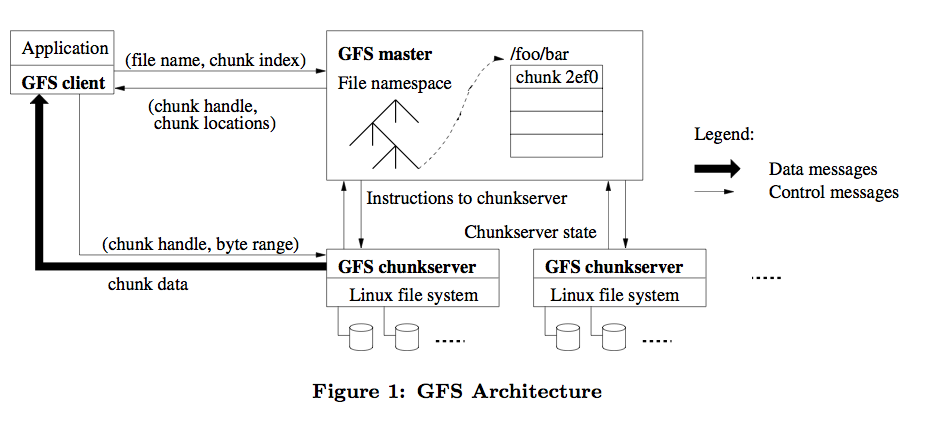
\includegraphics[scale=0.5]{images/gfs}
\caption{Architektura Google File System \cite{gfs}}
\label{fig:gfs}
\end{figure}

\section{BigTable}
Jedná se o systém na uchovávání dat společnosti Google, který je postavený nad Google File Systémem a jinými technologiemi společnosti Google. Jedná se o proprietární software, který není k dispozici mimo firmu Google vyjma možnosti využívat tento software jako část služby Google App Engine. V roce 2006 opět Google zveřejnil článek o BigTable \cite{bigtable}, avšak nyní s mnohem méně detaily nežli u svého článku o GFS \cite{gfs}, zřejmě z obav o přesné zkopírování jako u zmíněného systému. V době vydání článku BigTable obsluhoval více než 60 služeb firmy Google a škáloval několik petabytů dat na několika tisících počítačích. BigTable umožňuje využívání MapReduce frameworku. Jedná se o první implementaci mnohasloupcové, distribuované, multidimenzionální perzistentní seřazené mapy. Google opět udal trend, jakým se podobné systémy začaly ubírat. Datový model BigTable v budoucnu inspiroval i tvůrce Apache Cassandra, která je hlavním tématem této práce a proto detaily ohledně datového modelu prozatím přeskočíme.

\section{MapReduce}
Je programovací model a framework prvně představený společností Google \cite{mapreduce} na zpracování velkého datasetu. Uživatel specifikuje mapovací funkci, která zpracuje páry (klíč, hodnota) a vygeneruje přechodné páry (klíč, hodnota), které jsou pak předané redukční funkci, která sloučí všechny mezi-hodnoty se stejným mezi-klíčem. Mnoho příkladů z reálného světa lze převést do tohoto paradigmatu. Výhodou těchto funkcionálně napsaných programů je, že jsou automaticky dobře paralelizovatelné. Systém se stará o detaily distribuce dat a rozhození jednotlivých úloh na jednotlivé počítače a obsluhuje chyby a neočekávané stavy. Díky tomu umožňuje i programátorům s velmi malou znalostí paralelního programování napsat vysoce paralelní a efektivní programy. 

Toto paradigma se stalo nejdůležitějším stavebním kamenem pro zpracovávání BigData. Díky tomuto mechanismu jsme schopni zpracovávat terabyty dat rychle a efektivně a vypočítaný výsledek znovu uložit do databáze. Veškeré postupy zpracování BigData jsou přímo či nepřímo založené na MapReduce. Na obrázku \ref{fig:mapreduce} je tento mechanismus zobrazen, nejdříve jak vypadá mapovací a následně redukovací fáze, ze které vznikne konečný výsledek.

\begin{figure}[!h]
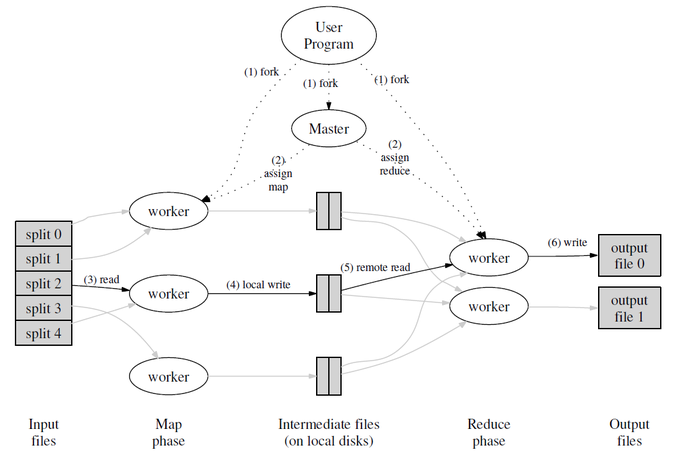
\includegraphics[scale=0.6]{images/mapreduce}
\caption{MapReduce schéma \cite{mapreduce}}
\label{fig:mapreduce}
\end{figure}

\newpage

\section{NoSQL}
Se zkratkou SQL se můžeme setkat u relačních databázových systémů. Zkratka NoSQL neznamená pravý opak, písmena \uv{No} znamenají \uv{Not Only}, tedy ne pouze. Jedná se o databázový koncept, který se vyskytuje u nerelačních databází. V tomto konceptu datové úložiště i zpracování dat používají jiné prostředky, než je běžné tabulkové schéma relační databáze. Výhodami tohoto konceptu jsou jednoduchý design a horizontální i vertikální škálovatelnost. NoSQL databáze často podporují také podmnožinu jazyka SQL. Většinou se jedná o jednoduché funkce, jako je vkládání a velice jednoduché výběry. Některé NoSQL databáze mají i velice odlišný ukládací model (například stromový či grafový), tím pádem je složitost pro různé operace odlišná. Nejčastější podobou NoSQL databáze jsou dvojice klíč-hodnota, čili mapa. Podle dosavadních informací lze říci, že Google BigTable je NoSQL databáze. Mezi charakteristiky NoSQL databází můžeme zahrnout

\begin{itemize}
\item \textbf{Datový a dotazovací model} - Jak již bylo řečeno, NoSQL databáze se liší způsobem udržování dat a dotazováním nad nimi.
\item \textbf{Perzistence} - Ne všechny NoSQL databáze ukládají svá data na disk, některé databáze běží pouze v operační paměti.
\item \textbf{Rozhraní} - Některé databáze komunikují skrze REST rozhraní a některé pomocí binárních protokolů. 
\item \textbf{BASE} - Tak jako relační databáze využívají vlastnosti ACID (Atomic Consistent Isolation Durability), tak v NoSQL je ekvivalentem BASE (Basically Available, Soft state, Eventual consistency), kde každá NoSQL databáze garantuje jednotlivé vlastnosti různými mechanismy a nastaveními nebo je databáze již od základu navržena s danými vlastnostmi.   
\end{itemize}


NoSQL databáze jsou dalším základním stavebním kamenem BigData. NoSQL databáze jsou často kompatibilní s MapReduce konceptem, čímž tvoří ideální dvojici pro uchovávání a zpracování velkého množství dat. 

